\documentclass[12pt, twoside]{article}
\usepackage[letterpaper, margin=1in, headsep=0.5in]{geometry}
\usepackage[english]{babel}
\usepackage[utf8]{inputenc}
\usepackage{amsmath}
\usepackage{amsfonts}
\usepackage{amssymb}
\usepackage{tikz}
\usetikzlibrary{quotes, angles}
\usepackage{graphicx}
\usepackage{enumitem}
\usepackage{multicol}

\newif\ifmeta
\metatrue %print standards and topics tags

\title{Regents Geometry}
\author{Chris Huson}
\date{September 2020}

\usepackage{fancyhdr}
\pagestyle{fancy}
\fancyhf{}
\renewcommand{\headrulewidth}{0pt} % disable the underline of the header
\raggedbottom


\fancyhead[LE]{\thepage}
\fancyhead[RO]{\thepage \\ Name: \hspace{4cm} \,\\}
\fancyhead[LO]{BECA / Dr. Huson / Geometry 07-Similarity\\* pset ID: 111}

\begin{document}

\subsubsection*{7-5HW-Symmetry}
\begin{enumerate}
\item After a dilation with center $(0,0)$, the image of $\overline{MN}$ is $\overline{M'N'}$. If $MN=7.2$ and $M'N'=36$, find the scale factor of this dilation. \vspace{3cm}

\item Circle YES or NO to indicate whether the given transformation maps the hexagon onto itself.
  \vspace{0.5cm}
  \begin{multicols}{2}
    \begin{enumerate}
    \item Yes \quad No \quad A rotation of $120^\circ$ counterclockwise around point $D$.
     \item Yes \quad No \quad A reflection over $\overleftrightarrow{AE}$
     \item Yes \quad No \quad A reflection over a line through the midpoints of  $\overline{BC}$ and $\overline{EF}$.
     \item Yes \quad No \quad A rotation of $60^\circ$ clockwise around the hexagon's center.
     \end{enumerate}
   \begin{center}
       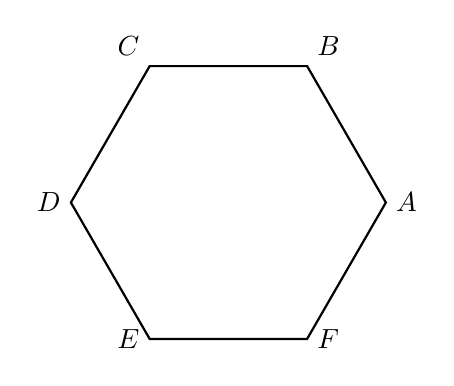
\begin{tikzpicture}%[scale=.48]
         \draw [thick]
         (0:2)node[right] {$A$}--
         (60:2)node[above right] {$B$}--
         (120:2)node[above left] {$C$} --
         (180:2)node[left] {$D$}--
         (240:2)node[left] {$E$}--
         (300:2)node[right] {$F$}--cycle;
       \end{tikzpicture}
     \end{center}
   \end{multicols} \vspace{0.5cm}

\item The line $l$ has the equation $y=-\frac{3}{5}x+4$. To each line below, circle whether $l$ is parallel, perpendicular, or neither.
    \begin{enumerate}
      \item parallel \quad perpendicular \quad neither \qquad $y=\frac{3}{5}x-2$
      \vspace{0.5cm}
      \item parallel \quad perpendicular \quad neither \qquad $y=\frac{5}{3}x+9$
      \vspace{0.5cm}
      \item parallel \quad perpendicular \quad neither \qquad $3x-5y=-15$
      \vspace{2cm}
      \item parallel \quad perpendicular \quad neither \qquad $5x-3y=6$
      \vspace{1.7cm}
    \end{enumerate}

\newpage
\item The figure shows a rectangle (not a square).
   \begin{center}
     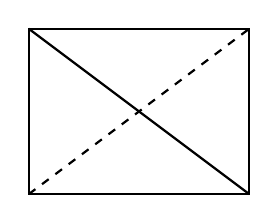
\begin{tikzpicture}[scale=0.7]
       \coordinate (A) at (0, 0); %[label=above left:$P$]
       \coordinate (B) at (4, 0);
       \coordinate (C) at (4, 3);
       \coordinate (D) at (0, 3);
       \draw [thick] (A)--(B)--(C)--(D)--cycle;
       \draw [thick, dashed] (A)--(C);
       \draw [thick] (B)--(D);
       %\draw [thick, xshift=2cm, yshift=2.5cm] (85:3);
     \end{tikzpicture}
   \end{center}
   Which transformations carries the rectangle onto itself? Mark each True or False.
     \begin{enumerate}
       \item A reflection over the solid diagonal \hfill True \quad False
       \item A reflection over the dashed diagonal \hfill True \quad False
       \item A clockwise rotation of $90^\circ$ about the intersection of the diagonals \hfill True \quad False
       \item A clockwise rotation of $180^\circ$ about the intersection of the diagonals \hfill True \quad False
     \end{enumerate}
     \vspace{1cm}

\item What is the smallest non-zero angle of rotation about its center that would map the pentagon onto itself? \vspace{0.25cm} %$ABCDE$
   \begin{center}
       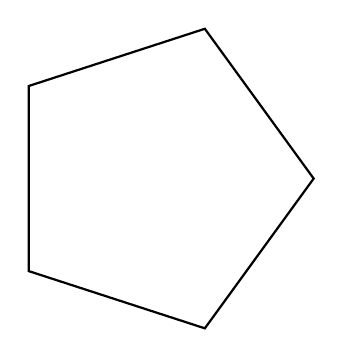
\begin{tikzpicture}%[scale=.48]
         \draw [thick]
         (0:2)--% node[right] {$A$}--
         (72:2)--% node[above right] {$B$}--
         (144:2)--% node[above left] {$C$} --
         (216:2)--% node[left] {$D$}--
         (288:2)--cycle;% node[right] {$E$}--cycle;
       \end{tikzpicture}
     \end{center} \vspace{0.5cm}

\item In the diagram below, the chords $\overline{AE}$ and $\overline{BD}$ intersect at $C$, with $\triangle ABC \sim \triangle DEC$, $BC=3$, $AC=4$, and $AE=11$. Determine the length of $\overline{CD}$.
      \begin{center}
      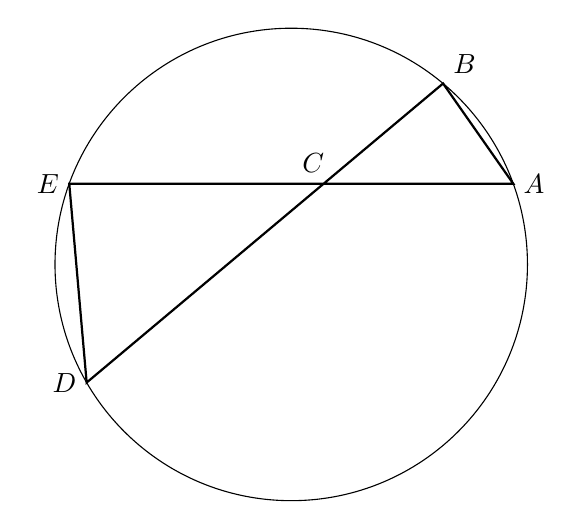
\begin{tikzpicture}[scale=.6]
        \draw (0,0) circle[radius=5];
        \draw [thick]
        (20:5) node[right] {$A$}--
        (160:5) node[left] {$E$}--
        (210:5) node[left] {$D$}--
        (50:5) node[above right] {$B$}--cycle;
        \draw (75:1.8) node[above] {$C$};
      \end{tikzpicture}
    \end{center}



\end{enumerate}
\end{document}